% ---------------------------------------------------------------------------- %
\subsection{Aufbau}
% ---------------------------------------------------------------------------- %

Das System besteht  aus zwei Teilen. Aus Sensoren, welche sich  direkt bei den
einzelnen Solarmodulen befinden und einer Zentrale (Masterger\"at), welche die
Informationen der Sensoren auswertet.

%\begin{figure}[h!]
%    \centering
%    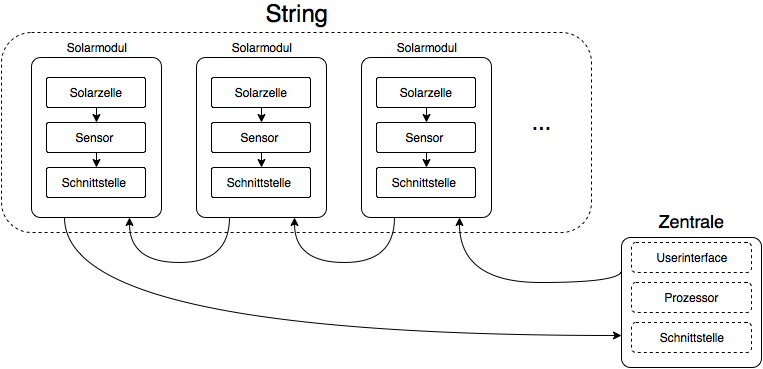
\includegraphics[width=.9\textwidth]{images/blockdiag.png}
%    \caption{Blockdiagramm Hardwareaufbau}
%    \label{fig:blockdiag:hardware}
%\end{figure}


% ---------------------------------------------------------------------------- %
\subsection{Spezifikationen}
\label{subsec:specs}
% ---------------------------------------------------------------------------- %

Die Spezifikationen  werden aufgegliedert gem\"ass den  beiden Hauptteilen des
Gesamtsystems: Sensor und Masterger\"at.

% ---------------------------------------------------------------------------- %
\subsubsection{Sensor}
% ---------------------------------------------------------------------------- %

\begin{minipage}[c][][t]{.49\textwidth}
	Der Sensor besteht  aus einer m\"oglichst kleinen  Leiterplatte, welche direkt
	bei den  einzelnen Modulen installiert  werden kann.

	Jeder  Sensor  \"uberwacht  dabei  die   Spannung  der  jeweiligen  Zelle  und
	\"ubermittelt  diese  in  vorgegebenen Zeitabst\"anden  an  die  Zentrale. Die
	Spannungsmessung  und  die  Kommunikation werden  von  einem  energiesparenden
	Mikrokontroller geregelt.

	F\"ur  die  Daten\"ubertragung   werden  keine  zus\"atzlichen  Installationen
	ben\"otigt. Die   Kommunikation   findet   \"uber   die   Stromleitungen   der
	Solaranlage   statt. Daf\"ur  ist   eine   Modulation  vorgesehen. F\"ur   die
	Realisierung werden  folgende zwei M\"oglichkeiten evaluiert  (siehe Abschnitt
	\ref{subsec:losungsvarianten}).

	\begin{itemize}
		\item
			kapazitiv eingekoppelte Frequenzumtastung (FSK)
		\item
			serielle \"Ubertragung durch kurzzeitiges Kurzschliessen der Zelle
	\end{itemize}

	Der     schematische    Aufbau     des     Sensors     ist    in     Abbildung
	\ref{fig:blockdiag:sensor} zu sehen.
\end{minipage}
\hspace*{0.02\textwidth}
\begin{minipage}[c][][t]{.49\textwidth}
		\centering
		\includegraphics[width=\textwidth]{images/blockdiag-sensor.png}
		\captionof{figure}{Blockdiagramm des Sensors}
		\label{fig:blockdiag:sensor}
\end{minipage}


\clearpage
% ---------------------------------------------------------------------------- %
\subsubsection{Masterger\"at}
% ---------------------------------------------------------------------------- %

\textbf{Supervisor}:
Die  Aufgabe   des  Supervisors  besteht   im  Empfangen  der   Messwerte  der
Panel-Sensoren  sowie der  Messung  des Stromes  der einzelnen  Strings. Diese
Informationen sollen gespeichert und verarbeitet werden um bei Bedarf Anwender
\"uber ein Display oder SMS zu  informieren und elektrische Signale via Relais
auszugeben.

\textbf{Hardware}:
Die  Grundlage  dieses   Ger\"ats  bildet  ein  Rechner   welcher  \"uber  die
ben\"otigten Schnittstellen  und Rechenleistung verf\"ugt. Aufgrund  der guten
Verf\"ugbarkeit,  g\"unstigen  Preises  und grosser  Auswahl  and  kompatibler
Peripherie wird hierf\"ur ein Raspberry Pi Modell B+ oder neuer eingesetzt. Es
kann  direkt mit  einem  Anzeigemodul verbunden  werden, hat  USB-Anschl\"usse
f\"ur ein USB-GSM Modem und ist  klein genug um in einem DIN-Schienengeh\"ause
untergebracht zu werden.

Funktionen,   welche   nicht   Bestandteil  des   komperziell   erh\"altlichen
Computermoduls  enthalten  sind  werden  auf einer  im  Verlauf  des  Projekts
entwickelten Tochterplatine realisiert. Dies sind inbesondere die Strommessung
der  Strings bis  10A,  der Empfang  von Nachrichten  der  Sensoren sowie  die
Ausgabe von Signalen via Relais.

Die  Stromversorgung  des  Ger\"ats   wird  von  einem  eingekauften  5V-Modul
\"ubernommen.

\textbf{Software}:
F\"ur  das Raspberry  Pi  sind angepasste  Versionen diverser  Betriebssysteme
verf\"ugbar. Das  am  besten  unterst\"utzte  ist eine  Variante  von  Debian,
genannt Raspbian. Diese bietet neben  grundlegenden Systemfunktionen auch eine
Vielzahl von  Programmbibliotheken, welche zur Entwicklung  von Auswertung und
Benutzerinterface von grossem Nutzen sind.
